\documentclass[sigconf]{acmart}

\usepackage{booktabs} % For formal tables
\usepackage{multirow}
\usepackage{listings}   

\usepackage{tikz}
\usetikzlibrary{automata,positioning}


\lstset{
  frame=none,
  language=scala,
  basicstyle={\small\ttfamily}
}

\sloppy

% Copyright
%\setcopyright{none}
%\setcopyright{acmcopyright}
%\setcopyright{acmlicensed}
\setcopyright{rightsretained}
%\setcopyright{usgov}
%\setcopyright{usgovmixed}
%\setcopyright{cagov}
%\setcopyright{cagovmixed}


% DOI
%\acmDOI{10.475/123_4}

% ISBN
%\acmISBN{123-4567-24-567/08/06}

%Conference
\acmConference[Scala 2018]{Ninth ACM SIGPLAN Symposium on Scala, 2018}{September 2018}{St. Louis, Missouri, United States}
\acmYear{2018}
\copyrightyear{2018}


%\acmArticle{4}
%\acmPrice{15.00}

% These commands are optional
%\acmBooktitle{Transactions of the ACM Woodstock conference}
%\editor{Jennifer B. Sartor}
%\editor{Theo D'Hondt}
%\editor{Wolfgang De Meuter}


\begin{document}
\title{Parser-Combinators for Context-Free Path Querying}
%\titlenote{This work is supported by grant from JetBrains Research.}
%\subtitle{Extended Abstract}
%\subtitlenote{The full version of the author's guide is available as
%  \texttt{acmart.pdf} document}


\author{Sophia Smolina}
\affiliation{%
  \institution{Electrotechnical University}
  \streetaddress{ul. Professora Popova 5,}
  \city{St. Petersburg}
  \country{Russia}
  \postcode{197376}
}
\email{sofysmol@gmail.com}

\author{Ekaterina Verbitskaia}
\affiliation{%
  \institution{Saint Petersburg State University}
  \streetaddress{7/9 Universitetskaya nab.}
  \city{St. Petersburg}
  \country{Russia}
  \postcode{199034}
}
\email{kajigor@gmail.com}

\author{Ilya Kirillov}
\affiliation{%
  \institution{Saint Petersburg State University}
  \streetaddress{7/9 Universitetskaya nab.}
  \city{St. Petersburg}
  \country{Russia}
  \postcode{199034}
}
\email{kirillov.ilija@gmail.com}

\author{Ilya Nozkin}
\affiliation{%
  \institution{Saint Petersburg State University}
  \streetaddress{7/9 Universitetskaya nab.}
  \city{St. Petersburg}
  \country{Russia}
  \postcode{199034}
}
\email{nozhkin.ii@gmail.com}


\author{Semyon Grigorev}
\orcid{0000-0002-7966-0698}
\affiliation{%
  \institution{Saint Petersburg State University}
  \streetaddress{7/9 Universitetskaya nab.}
  \city{St. Petersburg}
  \country{Russia}
  \postcode{199034}
}
\email{s.v.grigoriev@spbu.ru}

% The default list of authors is too long for headers.
\renewcommand{\shortauthors}{Smolina et al.}

\begin{abstract}
A transparent integration of a domain-specific language for specification of context-free path queries (CFPQs) into a general-purpose programming language as well as static checking of errors in queries may greatly simplify the development of applications utilizing CFPQs.  
Such techniques as LINQ and ORM can be used for the integration, but they have issues with flexibility: query decomposition and reusing of subqueries are a challenge.
Adaptation of parser combinators technique for paths querying may solve these problems. 
Conventional parser combinators process linear input and only the Trails library is known to apply this technique for path querying.
Trails suffers the common parser combinators issue: it does not support left-recursive grammars and also experiences problems in cycles handling.
We demonstrate that it is possible to create general parser combinators for CFPQ which support arbitrary context-free grammars and arbitrary input graphs.
We implement a library of such parser combinators and show that it is applicable for realistic tasks.
\end{abstract}

%
% The code below should be generated by the tool at
% http://dl.acm.org/ccs.cfm
% Please copy and paste the code instead of the example below.
%
\begin{CCSXML}
<ccs2012>
<concept>
<concept_id>10002951.10002952.10002953.10010146</concept_id>
<concept_desc>Information systems~Graph-based database models</concept_desc>
<concept_significance>500</concept_significance>
</concept>
<concept>
<concept_id>10002951.10002952.10003197.10010825</concept_id>
<concept_desc>Information systems~Query languages for non-relational engines</concept_desc>
<concept_significance>500</concept_significance>
</concept>
<concept>
<concept_id>10011007.10011006.10011008.10011009.10011012</concept_id>
<concept_desc>Software and its engineering~Functional languages</concept_desc>
<concept_significance>300</concept_significance>
</concept>
<concept>
<concept_id>10003752.10003766.10003771</concept_id>
<concept_desc>Theory of computation~Grammars and context-free languages</concept_desc>
<concept_significance>300</concept_significance>
</concept>
</ccs2012>
\end{CCSXML}

\ccsdesc[500]{Information systems~Graph-based database models}
\ccsdesc[500]{Information systems~Query languages for non-relational engines}
\ccsdesc[300]{Software and its engineering~Functional languages}
\ccsdesc[300]{Theory of computation~Grammars and context-free languages}

\keywords{Graph Databases, Language-Constrained Path Problem, Context-Free Path Querying, Parser Combinators, Generalized LL, GLL, Neo4J, Scala}

\maketitle

\section{Introduction}

Scalable high-performance graph analysis is an actual challenge.
There is a big number of ways to attack this challenge~\cite{Coimbra2021} and the first promising idea is to utilize general-purpose graphic processing units (GPGPU).
Such existing solutions, as CuSha~\cite{10.1145/2600212.2600227} and Gunrock~\cite{7967137} show that utilization of GPUs can improve the performance of graph analysis, moreover it is shown that solutions may be scaled to multi-GPU systems.
But low flexibility and high complexity of API are problems of these solutions.

The second promising thing which provides a user-friendly API for high-performance graph analysis algorithms creation is a GraphBLAS API~\cite{7761646} which provides linear algebra based building blocks to create graph analysis algorithms.
The idea of GraphBLAS is based on a well-known fact that linear algebra operations can be efficiently implemented on parallel hardware.
Along with that, a graph can be natively represented using matrices: adjacency matrix, incidence matrix, etc.
While reference CPU-based implementation of GraphBLAS, SuiteSparse:GraphBLAS~\cite{10.1145/3322125}, demonstrates good performance in real-world tasks, GPU-based implementation is challenging.

One of the challenges in this way is that real data are often sparse, thus underlying matrices and vectors are also sparse, and, as a result, classical dense data structures and respective algorithms are inefficient. 
So, it is necessary to use advanced data structures and procedures to implement sparse linear algebra, but the efficient implementation of them on GPU is hard due to the irregularity of workload and data access patterns.
Though such well-known libraries as cuSPARSE show that sparse linear algebra operations can be efficiently implemented for GPGPU, it is not so trivial to implement GraphBLAS on GPGPU. 
First of all, it requires \textit{generic} sparse linear algebra, thus it is impossible just to reuse existing libraries which are almost all specified for operations over floats.
The second problem is specific optimizations, such as masking fusion, which can not be natively implemented on top of existing kernels.
Nevertheless, there is a number of implementations of GraphBLAS on GPGPU, such as GraphBLAST~\cite{yang2019graphblast}, GBTL~\cite{7529957}, which show that GPGPUs utilization can improve the performance of GraphBLAS-based graph analysis solutions.
But these solutions are not portable because they are based on Nvidia Cuda stack.
Moreover, the scalability problem is not solved: all these solutions support only single-GPU, not multi-GPU computations.

To provide portable GPU implementation of GraphBLAS API we developed a \textit{SPLA} library\footnote{Source code available at: \url{https://github.com/JetBrains-Research/spla}}.
This library utilizes OpenCL for GPGPU computing to be portable across devices of different vendors.
Moreover, it is initially designed to utilize multiple GPGPUs to be scalable.
To sum up, the contribution of this work is the following.
\begin{itemize}
    \item Design of portable GPU GraphBLAS implementation proposed. The design involves the utilization of multiple GPUS. Additionally, the proposed design is aimed to simplify library tuning and wrappers for different high-level platforms and languages creation. 
    \item Subset of GraphBLAS API, including such operations as masking, matrix-matrix multiplication, matrix-matrix e-wise addition, is implemented. The current implementation is limited by COO and CSR matrix representation format and uses basic algorithms for some operations, but work in progress and more data formats will be supported and advanced algorithms will be implemented in the future.
    \item Preliminary evaluation on such algorithms as breadth-first search (BFS) and triangles counting (TC), and real-world graphs shows portability across different vendors and promising performance: for some problems Spla is comparable with GraphBLAST. Surprisingly, for some problems, the proposed solution on embedded Intel graphic card shows better performance than SuiteSparse:GraphBLAS on the respective CPU. At the same time, the evaluation shows that further optimization is required.
\end{itemize} 
\section{Задача о поиске путей с ограничениями в терминах формальных языков}


Что, откуда и зачем.

История вопроса.


\subsection{Постановка задачи }



Функция $\omega(\pi) = \omega((v_0, l_0, v_1),(v_1,l_1,v_2),\dots,(v_{n-1},l_n,v_n)) = l_0 \cdot l_1 \cdot \ldots \cdot l_n $ строит слово по пути посредством конкатенации меток рёбер вдоль этого пути.
Очевидно, для пустого пути данная функция будет возвращать пустое слово, а для пути длины $n  > 0$ --- непустое слово длины $n$.

Путь $G = \langle \Sigma, N, P \rangle$ --- контекстно-свободная граммтика.
Будем считать, что $L \subseteq \Sigma$.
Мы не фиксируем стартовый нетерминал в определении граммтики, поэтому, чтобы описать язык, задаваемый ей, нам необходимо отдельно зафиксировать стартовый нетерминал.
Таким образом, будем говорить, что $L(G,N_i) = \{ w | N_i \xRightarrow[G]{*} w  \}$ --- это язык задаваемый граммтикой $G$ со стартовым нетерминалом $N_i$.

Задача достижимости:

Задача поиска путей:

В задаче поиска путей мы можем накладывать дополнительные ограничения на путь (например, чтобы он был простым или кратчайшим), но это уже другая история.


\subsection{О разрешимости задачи}

Сведение к задаче о пересечениии с регулярным.

Замкнутость регулярных.

Проверка пустоты.

Замкнутость контекстно-свободных.
Проверка пустоты.

Про другие классы языков: конъюнктивные, булевы, многокомпонентные.

\subsection{Области применения}
Где применятеся

Статанализ.

Графовые БД.

Куча ссылок. Примеры?

\subsection{Вопросы и задачи}
\begin{enumerate}
  \item Пучть есть граф. Задайте грамматику дл поиска всех путей, таких, что....
  \item Существует ли в графе !!! путь из А в Б, такой что!!!
  \item Для графа !!! постройте все пути, удовлетворяющие !!!!

  \item Задача 1
  \item Задача 2
\end{enumerate}

\section{Generalized Parser Combinators}
\label{sec:GLL}

Combinators techniques are shown to be applicable for graph traversing~\cite{ScalaGraphParsing}, but it still suffers from the common issue with left-recursive definitions.
A general parser combinators library Meerkat~\cite{Meerkat}, implemented in the Scala programming language, removes this restriction by using memoization, continuation-passing style, and the ideas of Johnson~\cite{Johnson}.
Meerkat converts parsers into a memoized versions of themselves.
The memoization routine stores parsing results the first time they are computed and reuses them every time they are needed again.
Every time a new parsing result for some combinator is calculated, all the combinators, which are dependent on it, are recomputed.
This way Meerkat employs left-recursive parser combinators, and it is also crucial for the handling of the cycles in the input graphs.

Meerkat supports the arbitrary (left-recursive and ambiguous) context-free specifications; it also supports the specification of action codes and provides a \lstinline{syn} macro for custom handling of the recursive nonterminal descriptions.
Meerkat constructs the compact representation of the parse forest in the form of SPPF, which can be used for CFPQs results representation~\cite{GrigorevR16}.
The worst case time and space complexity of the solution are cubic.

A Meerkat specification of the language $\{a^n b^n \mid n \geq 1\}$ is \lstinline{val S = syn("a" ~ S.? ~ "b")}. Here \lstinline{syn} is a macro which creates a parser: for example, it transforms string literals into parsers for those strings. The tilde \lstinline{~} stands for a sequential parser combinator, and the question mark \lstinline{?} describes optional parsing. Other combinators available in the Meerkat library are shown in Table~\ref{table:combinators}.

It is shown in~\cite{GrigorevR16} that the Generalized LL parsing algorithm~\cite{scott2010gll} can be generalized to process CFPQs effectively and the query result can be finitely represented.
As the Meerkat library is closely related to the Generalized LL algorithm, it is also possible to adapt the Meerkat library for graph querying.
It can be done by providing a function for retrieving the symbols which follow the specified position and utilizing it in the basic set of combinators.
Details are described in the next section.

\subsection{SPPF}

Parsing of a string with respect to an ambiguous grammar can result in several derivation trees for a single string.
The set of derivation trees is named a \emph{derivation forest}.
To store a derivation forest efficiently, the generalized parsing algorithms utilize a \emph{Shared Packed Parse Forest} proposed by Joan Rekers~\cite{SPPF}.
The most efficient compact representation of derivation forests is a Binarized Shared Packed Parse Forest (we will abbreviate it to SPPF)~\cite{brnglr}.
The GLL algorithm, which employs this structure, achieves the worst-case cubic space complexity~\cite{gllParsingTree}.

Binarized SPPF is a directed graph, each node of which has one of the four types described below.
Almost every node of the SPPF is decorated with the \emph{extension}: a pair $(i, j)$ where $i$ is a start position of a substring derivable from the node and $j$---its end position.

\begin{itemize}
    \item A \textbf{terminal node} is labelled $(T, i, j)$.
    \item A \textbf{nonterminal node} is labelled $(N, i, j)$.
    This node denotes that there is at least one derivation $N \Rightarrow^*_G \omega[i \dots j-1]$---a substring of the input from the $i$-th to the $j$-th position.
    Every derivation tree for the given substring and nonterminal can be extracted by left-to-right top-down traversal of SPPF started from the respective node.
    \item An \textbf{intermediate node}: a special kind of node used for the binarization of the SPPF. These nodes are labelled with $(t,i,j)$, where $t$ is a grammar slot.
    \item A \textbf{packed node} is labelled $(N \rightarrow \alpha, k)$, where $k$ is a position in the input of the right end of the leftmost subtree of this node.
    A subgraph with the root in such node is, in turn, a parse forest for which the first production is $N \rightarrow \alpha$.
\end{itemize}


An example of SPPF is presented in Fig.~\ref{fig:sppf}.
We removed redundant intermediate and packed nodes for simplicity and to decrease the size of the figure.

SPPF finitely represents a possibly infinite set of paths in the context of the language-constrained graph querying~\cite{GrigorevR16}.
Since the SPPF stores derivation trees for all paths, it is useful for postprocessing and further understanding of the query results.
In static code analysis, for example, it is possible to map paths back onto the source code thus providing a human-readable result.
\section{Parser Combinators for Path Querying}
\label{sec:combinators}

Parser combinators is a way to specify both a language syntax and a parser for it in terms of higher-order functions. 
Parser in this framework is a function which consumes a prefix of an input and returns either a parsing result or an error if the input is erroneous. 
Parser combinators compose parsers to form more complex parsers. 
A parser combinators library usually provides a set of a basic parser combinators, such as a combinator of the sequential application of the choice, but there can also be user-defined combinators.
Most parser combinators libraries, including the Meerkat library, can only process the linear input---strings or some kind of streams.
We modify the Meerkat library to work on the graph input.

%Parser combinators provide a way to specify a language syntax in terms of functions and operations on them. 
%A parser in this framework is usually a function which consumes a prefix of an input and returns either a parsing result or an error if the input is erroneous. 
%Parsers can be composed by using a set of parser combinators to form more complex parsers. 
%A parser combinators library provides with a set of basic combinators (such as sequential application or choice), and there can also be user-defined combinators. 
%Most parser combinators libraries, including the Meerkat library, can only process the linear input --- strings or some kind of streams. 
%We extend the Meerkat library to work on the graph input.

The following ideas are at the core of the modification.
%Extension is based on some common ideas.


\begin{itemize}
\item The intersection of a context-free and a regular language is context-free. There are several constructive proofs of this fact.
The proposed solution is a yet another constructive proof with the SPPF as a user-friendly representation of the context-free grammar for the intersection.
\item Linear input can be regarded as a linear directed graph with symbols of the input labeling the edges.
\item A conventional parser moves a pointer in the input from the position $i$ to the position $i+1$ and creates a new state when token between $i$-th and $i+1$-th positions matches what is required in the grammar.
In case of graph processing, there are possibly multiple ways to move from the current vertex $i$ and it is possible to produce multiple new states.
Generalized parsing is designed to optimally handle the production of multiple new states thus it is suitable to handle graph processing.
\item Matching a token in the input can be viewed as a predicate, for example $p_c (x) = x == c$. 
We can generalize this observation allowing matching of an edge label of an arbitrary type with a predicate of some sort.
\item If vertices of the graph contain any data of interest, we can treat them in the similar fashion as the edges. We can also convert the input graph transforming vertices into edges and then querying the transformed graph.
\end{itemize}


%\begin{itemize}
%\item Intersection of context-free language and regular one is a context-free language and there are different constructive proves of this fact.
%Proposed solution is a yet another constructive prove and SPPF is a just user-friendly representation of result context-free grammar.
%\item Linear input is a simple case of graph: positions are vertices and tokens are edges labels.
%Each edge is going from position (vertex) $i$ to position (vertex) $i+1$.
%\item Parser can move pointer in input from position $i$ to position $i+1$ and create new state when token between $i$ to position $i+1$ matches with required in grammar.
%In case of graph processing there are more then one ways to go from current vertex $i$ and it is possible to get more then one new state.
%Generalized parsing is designed to optimally handle steps which produce multiple new states and can handle help to handle this situation.
%\item We can treat the fact that token in input matches with required token from grammar as a predicate.
%This observation may be generalized: we can pass through  edge if its label satisfies some predicate.
%This way we can flexibly handle labels of arbitrary types.
%\item Vertex may be converted to edge: all incoming edges are convert to oncoming into source of new edge, all outgoing are convert to outgoing from target of new edge.
%This way we can handle vertex and edge labelled graphs as edge labelled.
%\end{itemize}

Querying process in our library is inherited from generalized parsing and is done in two steps.
The first step is ``parsing'': the construction of the SPPF which contains all derivation trees for the paths satisfying syntactic constraints.
The second step is semantic actions application which retrieves the necessary additional data about the paths from the SPPF.

\subsection{The Set of Combinators}

We demonstrate the set of combinators by example: the input graph, which represents a map, is presented in fig.~\ref{fig:graph}.
There are some cities connected by one-way roads represented by the edges labeled $road\_to$.
Each city is labeled by its name and a country it belongs to.

% \begin{figure}[h]
% \includegraphics[width=0.45\textwidth]{graph}
% \caption{Example Input Graph of Roads}
% \label{fig:graph}
% \end{figure}

\begin{figure}[h]
\resizebox {0.45\textwidth} {!}
{
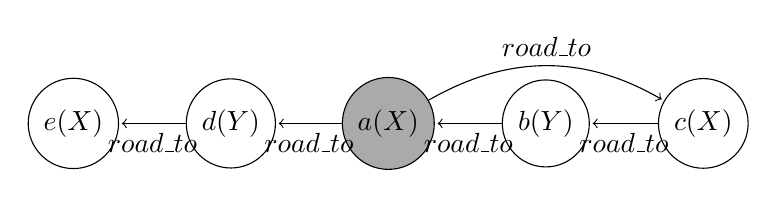
\begin{tikzpicture}[shorten >=1pt,node distance=2cm,on grid,auto] 
   \node[state] (a) [fill={rgb:black,1;white,2}]  {$a(X)$}; 
   \node[state] (b) [right=of a] {$b (Y)$}; 
   \node[state] (c) [right=of b] {$c (X)$}; 
   \node[state] (d) [left=of a] {$d (Y)$};
   \node[state] (e) [left=of d] {$e (X)$};
    \path[->] 
    (a) edge [bend left, above] node [above] {$road\_to$} (c)          
    (b) edge  node {$road\_to$} (a)
    (c) edge  node {$road\_to$} (b)
    (a) edge  node {$road\_to$} (d)
    (d) edge  node {$road\_to$} (e);
\end{tikzpicture}
}
\caption{Example graph. Vertex labels are in the form "city-name (country-name)"}
\label{fig:graph}
\end{figure}

Two basic building blocks of queries are the combinators for dealing with edges and vertices.
\begin{itemize}
    \item \lstinline{V[L](predicate: L =>   Boolean)} the combinator for processing vertices, where \lstinline{L} is a type of the node label. 
    Parsing with this combinator succeeds iff the vertex satisfies the predicate.
    \item \lstinline{E[N](predicate: N =>   Boolean)} the conbinator for processing edges, where \lstinline{N} is a type of the edge label. 
    Parsing with this combinator succeeds iff the edge satisfies the predicate.  
\end{itemize}

\begin{figure}[h]
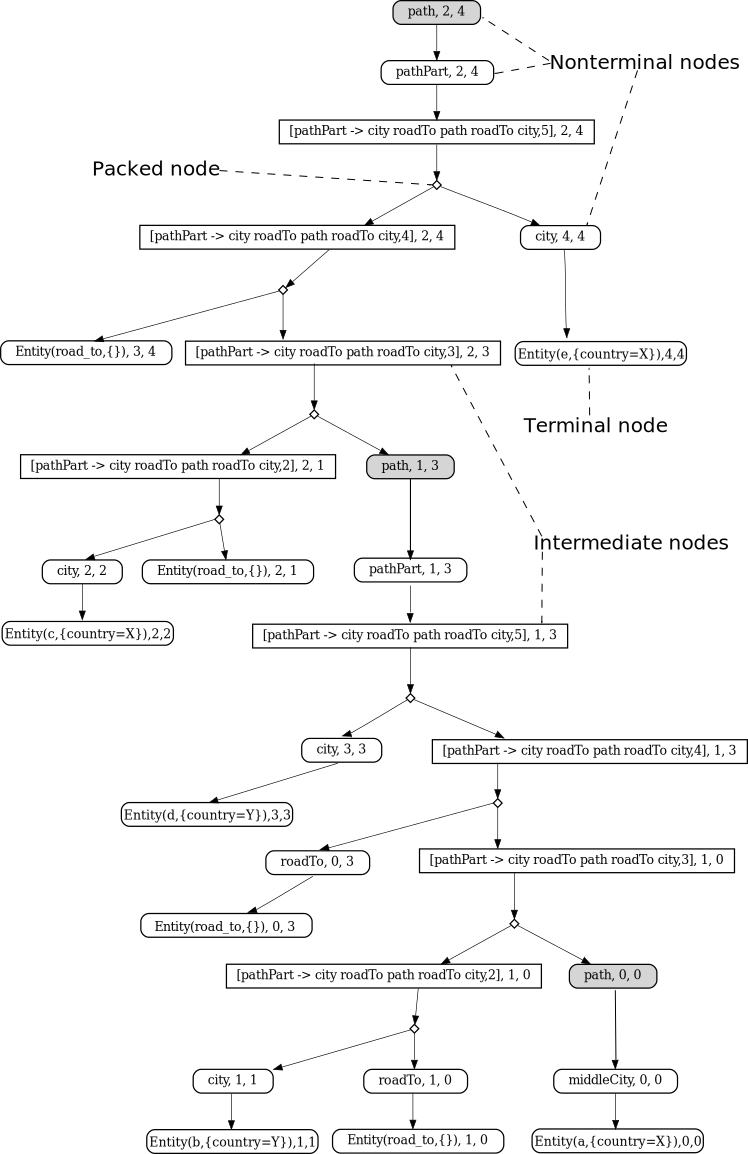
\includegraphics[width=0.49\textwidth]{sppf}
\caption{SPPF: result of applying cities query to the graph~\ref{fig:graph}}
\label{fig:sppf}
\end{figure}

To select cities which belong to some country, we can use the function \lstinline{V}: \lstinline{V[L]((e: Entity) =>   e.country =   "County Name")}.
Here \lstinline{Entity} is a property container for both edges and vertices. 
By using the \lstinline{Dynamic} trait, all accesses to properties (like \lstinline{(e: Entity).country}) are converted to the accesses to the properties of either a vertex or an edge.
For the sake of simplicity, we will omit \lstinline{Entity} type specifications for predicates. 
To query the graph for the paths from a city in the country $X$ to a city in the country $Y$, we need to sequentially compose the combinators for selecting the appropriate cities. 
A sequentialital combinator \lstinline{~} does just that: it sequentially  applies two queries one after the other. 
Let us denote a query for retrieving a city from the specific country \lstinline{city(name: String)} and a query for retrieving road edges \lstinline{roadTo}. 
With this denotation, a query \lstinline{city("X") ~ roadTo ~ city("Y")} returns the requested set of paths from the graph.
The complete query with all necessary subqueries is shown in fig.~\ref{fig:simpleQuery}.

\begin{figure}[h]
\begin{lstlisting}
def city(country: String) =
  V(_.country == country)
val roadTo = E(_.value() == "road_to")
val ourPath = 
  city("X") ~ roadTo ~ city("Y")
\end{lstlisting}
\caption{Path query}
\label{fig:simpleQuery}
\end{figure}

Having the query written, the next thing is to write a function to retrieve the actual data about the paths.
If we care only about the names of the cities, we can return a pair of the cities for each path.
First, we modify the query for vertices by adding the semantic action to it using the combinator \lstinline{^}: \lstinline{def city(name: String) =    syn(V(e.value() ==   name) ^ (_.value))}.
Then we need to actually map a path to a pair of cities: this is done with the combinator \lstinline{&}.
The complete query is in fig.~\ref{fig:simpleQueryV2}.
The result is the sequence of pairs of cities with the road between them.

%Now we would like to get all pair of cities which have a road between them. 
%So we need to transform our query to use semantic actions which is described in \ref{sec:semanticActions} section. 
%Now let us specify what we want from every our query. 
%From the \lstinline{city} query we want only city name, so we need to map a result of basic vertex combinator. 
%For that case we have a \lstinline{^} combinator we can write \lstinline{def city(name: String) = syn(V(e.value() == name) ^ (_.value))} to achieve  that. 
%In \lstinline{ourPath} query we need first and second cities to be represented as a pair. 
%For that we have a \lstinline{&} combinator which will map our sequence to a pair of strings.
%The final representation is shown on \ref{fig:simpleQueryV2}. 
%Now when we execute that query we will get a list which consists of all pairs of city's names which have a road between.

\begin{figure}[h]
\begin{lstlisting}
def city(country: String) =
  syn(V(_.country() == country) ^ (_.name))
val roadTo = E(_.value() == "road_to")
val ourPath = 
  syn(city("X") ~ roadTo ~ city("Y") &
    { case c0 ~ c1 => (c1, c2) })
\end{lstlisting}
\caption{Path query}
\label{fig:simpleQueryV2}
\end{figure}


The whole set of basic combinators, which our library provides, is presented in table~\ref{table:combinators}. 
There are two kind of combinators: the first kind combines parsers to form new parsers, meanwhile the second one is dedicated to the processing of the query result.
Whenever a string is used within a query, a parser which matches that string is implicitly generated.

\begin{table}[h]
\centering
\begin{tabular}{l@{}|l}
\multicolumn{1}{c|}{Combinator} & \multicolumn{1}{|c}{Description} \\ \hline
{\lstinline!a ~ b!} & sequential parsing: {\lstinline!a!} then {\lstinline!b!}   \\
{\lstinline!a | b!} & choice: {\lstinline!a!} or {\lstinline!b!}         \\
{\lstinline!a ?!}   & optional parsing: {\lstinline!a!} or nothing   \\
{\lstinline!a *!}   & repetition of zero or more {\lstinline!a!} \\
{\lstinline!a +!}   & repetition of at least one {\lstinline!a!} \\
{\lstinline!a ^ f!} & apply {\lstinline!f!} function to {\lstinline!a!} if  {\lstinline!a!} is a token \\
{\lstinline!a ^^!}  & capture output of {\lstinline!a!} if {\lstinline!a!} is a token    \\
{\lstinline!a & f!} & apply {\lstinline!f!} function to {\lstinline!a!} if  {\lstinline!a!} is a parser \\
{\lstinline!a &&!}  & capture output of {\lstinline!a!} if {\lstinline!a!} is a parser    \\
\hline
\end{tabular}
\caption{Meerkat combinators}
\label{table:combinators}
\end{table}


\subsection{Generic interface for input}
The combinators in our library are independent of the input representation. 
It is enough to specify two basic combinators which handle vertices and edges. 
Vertex handling is checking whether the vertex satisfies the given predicate.
In case of the edges, one needs to check which of the outgoing from the given vertex edges satisfy the given predicate. 
These two functions form the trait for the input (fig.~\ref{fig:input}).
It has two type parameters: the type of edge labels \lstinline{L} and the type of vertices labels \lstinline{N}.
We supported several different input sources:

%Combinators is a generic way to describe a query and when we have a query we want to execute that query on some graph considering it as an input for our query.
%The cool thing is that query execution mechanism may be fully separated from graph representation.
%We need only to have access to two very low-level functions, one for working with edges and one for vertices. 
%The first one would allow to get all edges outcoming from current vertex and also satisfies given predicate. 
%The second one will allow to check if current vertex satisfies given predicate.
%That interface is presented on fig~.\ref{fig:input}.
%It has two type parameters: \lstinline{L} for edge labels and \lstinline{N} for nodes.
%We have implementation of that input for the next data sources: 

\begin{itemize}
    \item Neo4jInput --- input source for the graph database Neo4j;
    \item GraphxInput --- input source for the graph presented in memory using GraphX library;
    \item LinearInput --- input source for the linear input data such as the ordinary strings.
\end{itemize}

\begin{figure}[h]
\begin{lstlisting}
trait Input[+L, +N] {
  def filterEdges(nodeId: Int, 
      predicate: L => Boolean): Seq[(L, Int)]
  def checkNode(nodeId: Int, 
      predicate: N => Boolean): Option[N]
}

\end{lstlisting}
\caption{Generalized input interface}
\label{fig:input}
\end{figure}

Since the required functions are simple, we believe it is possible to support most storages of graph-structured data.
Note, there are two technical limitations which arise from our decision to use values of the type \lstinline{Int} as unique identifiers for vertices (the \lstinline{nodeId} parameter).
It is impossible to correctly query the input graph with more than \lstinline{MAX_INT} vertices. 
Also there should be a way to provide such unique identifiers. Most systems already use unique identifiers by default, in other cases this feature can be implemented by the user.

%As far as required functions is very simple, we hope that this interface can be implemented for arbitrary storage of graph-structured data.
%Note, that currently we use \lstinline{Int} as unique identifier for nodes (the \lstinline{nodeId} parameter).
%It may be a technical restriction by the next two reason.
%\begin{itemize}
%\item It is impossible to use our library for correct processing of graph with more then \lstinline{MAX_INT} nodes. 
%\item It is necessary to provide such identifiers. Many systems use unique identifiers by default, but in some cases it may be necessary to implement required functionality manually.
%\end{itemize}



\subsection{Semantic Actions}
\label{sec:semanticActions}

Every path, which the query produces, has a derivation tree stored in the SPPF. 
The derivation tree is a very reach structure which can be hard to understand. 
To retrieve the data actually useful for the user, the library provides a mechanism of semantic actions. 
It is a way to apply some function to a parsed token or a subsequence. 

%Each path query produces a parse result stored in SPPF.
%This representation is very rich but hard to use and understand.
%That is why our library provides a mechanism which allows you to extract and process any useful data stored in parse result.
%This mechanism is called semantic actions.
%In general, they give you an opportunity to apply any function to parsed token or sequence.
%Now, let's understand how actions can be used in queries and how they are implemented in our library.

Semantic action binder for the tokens---vertices and edges alike---is \lstinline{^}. The most common use for it is to extract properties from the token and combine them in some fashion. 

%There are two main semantic action binders \lstinline{^} and \lstinline{&}.
%First of them is used when we need to perform some action on primitive tokens such as vertices or edges.
\begin{lstlisting}
// Defined in Terminal[+L] (edge) parser
def ^[U](f: L => U) = 
  new SymbolWithAction[L, Nothing, U] {...
  
// Defined in Vertex[+N] parser
def ^[U](f: N => U) = 
  new SymbolWithAction[Nothing, N, U] {...
\end{lstlisting}

For the combination of parsers there is a \lstinline{&} binder. Being  applied to a sequence of tokens, it can collect and process the data returned by the terminal parsers.
%Second is used when we need to process a result of combination of parsers.
\begin{lstlisting}
// Defined in Symbol[+L, +N, +V] parser
def &[U](f: V => U) = 
  new SymbolWithAction[L, N, U] {...
\end{lstlisting}

They both produce a new parser that parses the input exactly like the given parser but also have a bound function.
The function is referenced in each SPPF node produced by the corresponding parser.

%But actually, they both have the same behaviour, they produce a new parser that has the same parsing possibilities as an original parser but also have a binded function.
%Then, every SPPF node that will be produced by parser with binded function will have a reference to this function too.

%These binders along with the other combinators 

%So, these operations in composition with other combinators provides an instrument for data processing on which most queries are based. 
%For example, \lstinline{^} can extract some data from tokens and \lstinline{&} applied to sequence of tokens can collect and process data returned by terminal parsers.

The way semantic actions are executed has mostly remained the same as in the original Meerkat library: semantic actions are first executed for the children of the current node, then the results are collected and passed to a semantic action of the current node. 
If there are ambiguous nodes in the SPPF, the original Meerkat library just throws an exception. 
In our case, ambiguity can arise not only when there are multiple derivations of a string but ambiguous nodes can also represent several different subpaths which are derived from the respective nonterminal.
We chose to provide a way to extract the derivation trees from the SPPF lazily, since the number of the paths can be infinite. 
Unambiguous trees are yielded with a breadth-first search.


%The main idea of execution of semantic actions remained the same as in the original Meerkat library excepting one aspect.
%For each node we still just execute all actions of its children, collect results and pass them as argument to current function.
%But what should executor do if SPPF has ambiguous nodes? 
%Previous implementation just throws an exception in that case and it is reasonable because original library is written for linear parsing and most grammars allows disambiguation in that case.

%However, even unambiguous grammar can produce ambiguous derivations during parsing of graphs.
%That's why we provide a feature that makes it possible to extract ``all'' trees stored in SPPF.
%The number of path deriving from given grammar can be infinite, for example, when graph has cycles.
%This reason we can provide only a lazy stream of trees that allows to take as much of them as you need.
%Our solution is based on breadth first search that yields an unambiguous SPPF corresponding to some derivation immediately after it was found.

The composition of the extraction of trees and the semantic action execution is called \lstinline{executeQuery}.
It parses the input graph from all positions, produces a list of SPPF roots, extracts all derivations from every root, executes semantic actions and returns a lazy stream of results.
\section{Examples}
\label{sec:examples}

In this section, we describe some examples of queries written with the library proposed.
We show that the combinators are expressive enough for realistic queries and also ease their creation.

\subsection{Complicated Query to Map}

We would like to search for all the routes which pass through a fixed city $a$ such that the countries of the cities on the route form a palindrome.
This means that if a route starts at the city of the country $X$, then the last visited city should also belong to the country $X$.
We also demand that the fixed city $a$ is in the middle of the route.
This query can be written as shown in Fig.~\ref{fig:pathQuery}.
A combinator \lstinline{reduceChoice} reduces a list of queries to a single query by means of the combinator \lstinline{|}.
The implementation of the \lstinline{reduceChoice} is straightforward and can be found in Fig.~\ref{fig:reduceChoice}.
A subquery \lstinline{middleCity} matches the fixed city $a$ and a query \lstinline{roadTo} matches a \emph{roadTo} edge.

\begin{figure}[h]
\begin{lstlisting}
val countriesList = List("X", "Y")
val path =
  (reduceChoice(countriesList.map(pathPart)) |
    middleCity)
def pathPart(country: String) =
  syn(city(country) ~ roadTo ~ path ~
    roadTo ~ city(country))

val middleCity = V(_.value() == "a")
val roadTo = E(_.value() == "road_to")
def city(country: String) = V(_.country == country)
\end{lstlisting}
\caption{Path query}
\label{fig:pathQuery}
\end{figure}

\begin{figure}[h]
\begin{lstlisting}
def reduceChoice(xs: List[Nonterminal]) =
  xs match {
   case x :: Nil => x
   case x :: y :: xs =>
      syn(xs.foldLeft(x | y)(_ | _))
 }
\end{lstlisting}
\caption{Reduce choice function implementation}
\label{fig:reduceChoice}
\end{figure}

\begin{figure}[h]
\begin{lstlisting}
val middleCity =
  syn(V(_.value() == "a") ^^) & (List(_))
def pathPart(country: String) = syn(
  (city(country) ~ roadTo ~
    path ~ roadTo ~ city(country) & {
     case a ~ (b: List[_]) ~ c => a +: b :+ c})
\end{lstlisting}
\caption{Fixed queries}
\label{fig:fixedPathQ}
\end{figure}

To filter out all the data but the list of the cities on the route, we can add the semantic actions as shown in Fig.~\ref{fig:fixedPathQ}


Executing the query for the graph in Fig.~\ref{fig:graph} returns the only three routes, which satisfy our restrictions.

\begin{itemize}
\item single-vertex path $a$;
\item $b \rightarrow a \rightarrow d$
\item $c \rightarrow b \rightarrow a \rightarrow d \rightarrow e$
\end{itemize}

A simplified SPPF for this query is presented in Fig.~\ref{fig:sppf}. Rounded rectangles represent nonterminals and other rectangles represent productions.
Every rectangle vertex contains a nonterminal name or a production rule, as well as the start and the end nodes in the input graph for the path derived from the corresponding SPPF vertex.
The start nonterminals are drawn in grey.

\subsection{Same Generation Query}

The generalization of the classical same generation query benefits from utilizing the first-order functions for querying.
Such a query can be used for the hierarchy analysis in RDF storages~\cite{CFGonRDF}.
Let's consider RDF graphs which have two pairs of relations between objects: (\emph{subClassOf}; $\text{\emph{subClassOf}}^{-1}$) and (\emph{type}; $\text{\emph{type}}^{-1}$). Each relation has its reverse denoted by the $-1$ superscript.
To search for the vertices which are on the same level of hierarchy one can use the grammars $G_1$~(Fig.~\ref{grammarQ1}) and $G_2$~(Fig.~\ref{grammarQ2}).

\begin{figure}[h]
   \centering
   \[
\begin{array}{rlcl}
   & S &  \rightarrow & \text{\textit{subClassOf}}^{-1} \ S? \ \text{\textit{subClassOf}} \\
   &   & |            & \text{\textit{type}}^{-1} \ S? \ \text{\textit{type}} \\
   % & S \rightarrow \text{\textit{subClassOf}}^{-1} \ \text{\textit{subClassOf}} \\
   % & S \rightarrow \text{\textit{type}}^{-1} \ \text{\textit{type}} \\
\end{array}
\]
   \caption{Context-free grammar $G_1$ for query 1}
   \label{grammarQ1}
   \end{figure}

\begin{figure}[h]
   \centering
   \[
\begin{array}{rlcl}
   & S & \rightarrow & B? \ \text{\textit{subClassOf}} \\
   % & S \rightarrow \text{\textit{subClassOf}} \\
   & B & \rightarrow & \text{\textit{subClassOf}}^{-1} \ B? \ \text{\textit{subClassOf}} \\
   %  & B \rightarrow \text{\textit{subClassOf}}^{-1} \ \text{\textit{subClassOf}} \\
\end{array}
\]
   \caption{Context-free grammar $G_2$ for query 2}
   \label{grammarQ2}
   \end{figure}


\begin{figure}[h]
\begin{lstlisting}
val query1: Nonterminal = syn(
   "subclassof-1" ~ query1.? ~ "subclassof" |
   "type-1" ~ query1.? ~ "type")
\end{lstlisting}
\caption{The same generation query (Query 1) in Meerkat}
\label{fig:query1Meerkat}
\end{figure}


\begin{figure}[h]
\begin{lstlisting}
val S = syn("subclassof-1" ~ S ~ "subclassof")
val query2 = syn(S ~ "subclassof")
\end{lstlisting}
\caption{The same generation query (Query 2) in Meerkat}
\label{fig:query2Meerkat}
\end{figure}

These two queries are context-free, so they can be easily written in Meerkat: the code is presented in Fig.~\ref{fig:query1Meerkat} and Fig.~\ref{fig:query2Meerkat}.

The implementations of the queries are similar and we can get rid of the code duplication by generalizing them.
The function \lstinline{sameGen} presented in Fig.~\ref{fig:gen} generalize the same generation query and is independent of the environment such as the input graph structure or other parsers.
Other queries can be written with this function, including the one presented in Fig.~\ref{fig:query1Meerkat}: it is the result of the application of \lstinline{sameGen} to the appropriate relations (which can be treated as the opening and closing brackets).
Another application of the \lstinline{sameGen} is the Query 2, presented in Fig.~\ref{fig:query2Gen}.

\begin{figure}[h]
\begin{lstlisting}
def sameGen(brs) =
  reduceChoice(
    bs.map {case (lbr, rbr) =>
      lbr ~ syn(sameGen(bs).?) ~ rbr})
\end{lstlisting}
\caption{Generic function for the same generations query}
\label{fig:gen}
\end{figure}


\begin{figure}[h]
\begin{lstlisting}
val query1 = syn(sameGen(List(
    ("subclassof-1", "subclassof"),
    ("type-1", "type"))))
\end{lstlisting}
\caption{Query 1 as an application of \lstinline{sameGen}}
\label{fig:query1Gen}
\end{figure}


\begin{figure}[h]
\begin{lstlisting}
val query2 = syn(
  sameGen(List(("subclassof-1", "subclassof"))) ~
   "subclassof")
\end{lstlisting}
\caption{Query 2 as an application of \lstinline{sameGen}}
\label{fig:query2Gen}
\end{figure}


We illustrated that the generic queries are easily written by means of the parser combinators.
It is possible to create a library of \ standard templates for most popular generic queries, such as the same generation query or other domain-specific queries (for example, for specific static code analysis problem).


\subsection{Classical Movies Queries}

We also implemented some queries to the movie database used in the Neo4j tutorial~\footnote{The set of classical queries to movie dataset in Cypher language: \url{https://neo4j.com/developer/movie-database/}.}.
The database contains the data about movies, actors, directors and the relations between them.
In this set of queries we demonstrate more semantic actions for the results processing.

Several helper functions were implemented to simplify the processing of the nodes and the edges.
They are built upon the basic combinators and are presented in Fig.~\ref{fig:helpers}.

\begin{figure}[h]
\begin{lstlisting}
def LV(labels: String*) =
  V(e => labels.forall(e.hasLabel))
def outLE(label: String) =
  outE(_.label() == label)
def inLE(label: String) =
  inE(_.label() == label)
\end{lstlisting}
\caption{Helpers for edges and nodes processing}
\label{fig:helpers}
\end{figure}

Having the helper functions implemented, we can start building queries.
The first query is selects \emph{actors who played in some film}.
Let us compare the Cypher (Fig.~\ref{fig:Q1_C}) and the Meerkat versions (Fig.~\ref{fig:Q1_M}) of this query.
The structure of them both is similar: the first part is a path specification and the second part is a specification of the value to return; in the Meerkat version we use semantic actions to calculate it.

\begin{figure}[h]
\begin{lstlisting}
MATCH (m:Movie {title: 'Forrest Gump'})
      <-[:ACTS_IN]-(a:Actor)
RETURN a.name, a.birthplace;
\end{lstlisting}
\caption{The query \emph{actors who played in some film} in Cypher}
\label{fig:Q1_C}
\end{figure}


\begin{figure}[h]
\begin{lstlisting}
val query =
  syn((
    (LV("Movie")::V(_.title == "Forrest Gump")) ~
    inLE("ACTS_IN") ~
    syn(
      LV("Actor") ^ (e =>
        (e.name,
          if (e.hasProperty("birthplace"))
            e.birthplace
          else "")))) &&)

executeQuery(query, input).foreach(println)
\end{lstlisting}
\caption{The query \emph{actors who played in some film} in Meerkat}
\label{fig:Q1_M}
\end{figure}


In the \emph{most prolific actors} query (Fig.~\ref{fig:Q2_C}) we need to use the postprocessing of the paths set to express ordering: \lstinline{executeQuery} returns a lazy set of paths which can be processed by using standard Scala functions as shown in Fig.~\ref{fig:Q2_C}.

\begin{figure}[h]
\begin{lstlisting}
MATCH (a:Actor)-[:ACTS_IN]->(m:Movie)
RETURN a, count(*)
ORDER BY count(*) DESC LIMIT 10
\end{lstlisting}
\caption{The query \emph{most prolific actors} in Cypher}
\label{fig:Q2_C}
\end{figure}


\begin{figure}[h]
\begin{lstlisting}
val query =
  syn((
    syn(LV("Actor") ^^) ~
    outLE("ACTS_IN") ~
    LV("Movie")) & (a => (a.name, a.toInt)))

executeQuery(query, input)
  .groupBy {case (a, i) => i}
  .toIndexedSeq
  .map {case (i, ms) => (ms.head._1, ms.length)}
  .sortBy {case (a, mc) => -mc}}
  .take(10)
  .foreach(println)

\end{lstlisting}
\caption{The query \emph{most prolific actors} in Meerkat}
\label{fig:Q2_C}
\end{figure}

For query presented in Fig.~\ref{fig:Q4_C} it is necessary to use subqueries.
First of all, we specify the \lstinline{user} subquery to find the user with the specific login.
Then we specify the \lstinline{friendsWith} subquery.
Finally, we combine these subqueries to form the resulting query.

\begin{figure}[h]
\begin{lstlisting}
MATCH (u:User {login: 'adilfulara'})-
      [:FRIEND]-(f:Person)-[r:RATED]->(m:Movie)
WHERE r.stars > 3
RETURN f.name, m.title, r.stars, r.comment;
\end{lstlisting}
\caption{The query \emph{mutual friend recommendations} in Cypher}
\label{fig:Q4_C}
\end{figure}


\begin{figure}[h]
\begin{lstlisting}
val user = syn(
  LV("User")::V(_.login == "adilfulara"))

val friendsWith =
  syn(inLE("FRIEND") | outLE("FRIEND"))

val query = syn((
  user ~ friendsWith ~ syn(LV("Person") ^^) ~
  syn(outLE("RATED") ^^) ~ syn(LV("Movie") ^^)) &
    {case p ~ r ~ m =>
       (p.name,
        m.title,
        r.stars.toInt,
        if (r.hasProperty("comment")) r.comment
        else "")})

executeQuery(query, input)
  .filter {case (_, _, s, _) => s > 3}
  .foreach(println)

\end{lstlisting}
\caption{The query \emph{mutual friend recommendations} in Meerkat}
\label{fig:Q4_M}
\end{figure}

%Finally we present composition of all abilities.
We also can compose all of the features used in the last two queries.
To express query presented in Fig.~\ref{fig:Q3_C}, we need to use not only postprocessing but also subquerying with postprocessing.
First, we evaluate the \lstinline{directors} subquery and build \lstinline{directorsMap} which is further used in the semantic actions for the \lstinline{actor_prof_director} subquery.
In the posprocessing step of the \lstinline{directors} subquery, we implement the filtering which relates to \lstinline{WHERE length(directed) >= 2} condition of the Cypher query.
In order to get the final result, we also need to use postprocessing as far as it is necessary to implement the filtering and sorting.

\begin{figure}[h]
\begin{lstlisting}
MATCH (a:Actor:Director)-[:ACTS_IN]->(m:Movie)
WITH a, count(1) AS acted WHERE acted >= 10
WITH a, acted
   MATCH (a:Actor:Director)-[:DIRECTED]->(m:Movie)
WITH a, acted, collect(m.title)
   AS directed WHERE length(directed) >= 2
RETURN a.name, acted, directed
ORDER BY length(directed) DESC, acted DESC;
\end{lstlisting}
\caption{The query \emph{Directed more than 2 films, acted in more than 10} in Cypher}
\label{fig:Q3_C}
\end{figure}


\begin{figure}[h]
\begin{lstlisting}
val directors = syn((
  syn(LV("Actor", "Director") ^^) ~
  outLE("DIRECTED") ~ LV("Movie")) & (_.id.toInt))

val directorsMap = executeQuery(directors, input)
  .groupBy(i => i)
  .map {case (i, ms) => (i, ms.length)}
  .filter {case (_, ms) => ms >= 2}

val actor_prof_director =  syn(
  LV("Actor", "Director") ::
    V(e => directorsMap.contains(e.id.toInt)) ^^)

val acts = syn(
  (actor_prof_director ~ outLE("ACTS_IN") ~
    LV("Movie")) & (a => (a.name, a.id.toInt)))

executeQuery(acts, input)
  .groupBy {case (a, i) => i}
  .toStream
  .map {case (i, ms) => (i, ms.head._1, ms.length)}
  .filter {case (i, a, mc) => mc >= 10}
  .map {case (i, a, mc) => (a, mc, directorsMap(i))}
  .sortBy {case (a, mc, dc) => (-dc, -mc)}
  .foreach(println)

\end{lstlisting}
\caption{The query \emph{Directed more than 2 films, acted in more than 10} in Meerkat}
\label{fig:helpers}
\end{figure}

This shows that our library is expressive enough to formulate realistic queries.
The main drawback of our library as compared to the Cypher language is that all additional logic such as
filtering, sorting or grouping has to be implemented manually as a separate step.
\section{Evaluation}

This section describes the methodology and answers the following research questions.

\begin{enumerate}
    \item Does fusion via distillation give any benefits at the software and hardware levels?
    \item What are the properties of the generated hardware?
    \item Does the generated hardware outperform software implementations?
\end{enumerate}

\subsection{Methodology}

Our focus is on creating a basis for future research and experiments, thus we make our experiments as much reproducible as possible\footnote{\url{https://github.com/sedwards-lab/fhw/tree/sparse-linear-algebra-distillation/examples/QTreeBenchmarks/diploma/verilog-bool-no-nnz-inlined} (online; accessed:
2022-06-07) Here one could find all the results. For each benchmark all statistics are specified: matrix names, their sizes, collected metrics for both hardware and software benchmarks.}. We benchmarked the following list of chained functions. The choice is prompted by the current state of the distiller: at the moment, it does not successfully distill matrix multiplication. However, the functions are still practical enough, for example, chained addition could be seen in Luby's maximal independent set algorithm and clearly describe the applicability of the proposed approach.

\begin{itemize}
    \item \mintinline{Haskell}{mAdd (==False) (||) (mAdd (==False) (||) m1 m2) m3}
    \item \mintinline{Haskell}{mask (mAdd (== False) (||) m2 m3) (m1)}
    \item \mintinline{Haskell}{map (==Zero) (to_nat) (mAdd (==False) (||) m1 m2}
    \item \mintinline{Haskell}{map (==Zero) (to_nat) (kron (==False) (&&) m1 m2}
\end{itemize}

Above, \mintinline{Haskell}{Zero} and \texttt{to\_nat} are corresponding definitions for Peano arithmetics, since the \texttt{.pot} language does not have any primitives. For the same reason, we operated with boolean matrices. Such functions could be abstracted with free variables and then instantiated in the emitted Haskell code. However, to get maximum from distillation, we provided all the information about the functions. 

For these functions, we compared the execution time of distilled and not distilled hardware generated circuits, execution time of original and distilled Haskell code and reference \textit{Suite Sparse}\footnote{\url{https://github.com/DrTimothyAldenDavis/GraphBLAS} (online; accessed:
2022-06-07), Suite Sparse library sources.}\textsuperscript{,}\footnote{The library also uses different variations of coordinate formats (opaque to the user) and not a quadtree representation.} variants of these functions in C\texttt{++}. Note that SuiteSparse does not support recursive data types, thus only the first two function chains were implemented in SuiteSparse (since Peano number is essentially a linked list). We did not replace Peano numbers with integers, so our experiments could be interpreted easier. For hardware experiments we collected execution time and the number of memory writes and reads, to access how well fusion is performed. For software experiments we only measured the execution time. Also note that we measured only the time, required to execute the lines above, not including any IO, required to get and evaluate function arguments. But in hardware benchmarks we measured the time required to pass arguments into the circuit's memory, because such IO is inevitable. It is tricky to make such measures in Haskell due to laziness, thus the programs were compiled with \texttt{--fno-full-laziness} to turn off memoization. Also all the arguments were forced to normal form via \texttt{force} and \texttt{evaluate}. Haskell programs were compiled\footnote{GHC 8.10.4.} with \texttt{-O2 --fno-full-laziness} and Suite Sparse was compiled with default flags and linked as a shared library to C\texttt{++} code.

We took matrices from SuiteSparse matrix collection with sizes ranging from \texttt{64x64} to \texttt{512x512}. We limited ourselves with such sizes due to the fact that this is the maximum sizes that fit into \texttt{bram} with $2^{16}$ address space. Such number of \texttt{bram} blocks is available only on really expensive FPGA boards, thus in practice sizes would be smaller to achieve better utilization. Once again, it models the situation when data fits into the cache, since \texttt{bram} in our circuits will operate as a cache in real application.

\subsection{Experiments}

Table~\ref{tab:bench_results} shows the results of all execution time benchmarks. To evaluate execution time for hardware simulation, implementation stage was performed to assess the maximum frequency of FPGA device used for synthesis and implementation, and the number of execution cycles was multiplied by the number of nanoseconds a clock cycle takes. The frequencies were equal within the same benchamark set, i.e., frequency was not affected by distillation. We used \texttt{xcu250figd2104-2L} device\footnote{\url{https://www.xilinx.com/products/boards-and-kits/alveo/u250.html}  (online; accessed:
2022-06-07)} for synthesis and implementation stages. It is not really a casual and affordable chip, but it contains enough \texttt{bram} for our evaluation to see scalability. In the table a median across several benchmarks is shown. 

As it could be seen, distillation steadily increases performance: up to 2x speedup for hardware simulation and up to 3x for software benchmarks. The results are maintained within the borders of the corresponding confidence interval and the borders are not shown for brevity. Hardware speedup is lower due to the different execution semantics, dataflow is not reduction-based and distillation is a reduction-based transformation. Note that generated hardware appears to be less performant than both Haskell and C\texttt{++}, which a bit contradicts the results from~\cite{oldfhw}. For hardware benchmarks \texttt{time (IO)} shows the execution time including the time needed to transfer the data though the arguments, \texttt{time (no IO)} does not include it in its turn. It could be seen that not all the benchmarks are computationally extensive enough to cover memory transferring costs, but for more complex examples the ratio would be better. Since we basically transfer the matrices node by node from a file in the testbench, we have probably the lowest possible latency, and in practice it would be higher if reading from DDR, however the bandwidth could be increased. Noticeably, running times for \texttt{mMaskAdd} for C\texttt{++} and distilled Haskell are similar, which shows that fusion really provides some extra performance: SuiteSparse at the moment does not implement any fusion.

Table~\ref{tab:mem_results} summarizes the ratios between distilled and not distilled hardware circuits memory reads and writes. Since in general case distillation removes extra pattern matching, essentially it saves memory reads and writes. The eventual number of memory reads and writes is implementation dependent, thus the table shows what share of speedup is prompted by saving memory operations. Distillation successfully reduces the number of memory accesses, about 15\% on average. \texttt{mMapKron} has a bit higher ratio due to the fact that \texttt{Nat} numbers require additional memory accesses, since the type is recursive. It could also be seen that a major part of speedups is attributed to saved memory accesses. 

Finally, table~\ref{tab:resource_util} shows device resources utilization ratios between distilled and not distilled hardware circuits and frequencies. Columns are device primitives: registers, lookup tables, \texttt{bram} blocks or multiplexers. Utilization for both types of circuits is below 1\% of available resources on the device, except for the memory. Memory blocks utilization is about 30\% (since we choose larger \texttt{brams} to store larger matrices). Apart from that, distilled circuits could have both higher and lower utilization. Since the hardware generation is primarily syntax-directed it follows from the distilled program structure. For example, distillation might glue two recursive functions into one (in that case, memory utilization would be lower, because each cluster of mutually recursive functions possesses its own heap) or make more recursive functions than in the original program. The frequencies are the same, however, they possibly could be made better with more intelligent buffer allocation.

\subsection{Discussion}
Answering the research questions above.

\begin{enumerate}
    \item Fusion gives significant benefits, however at the hardware level the benefits are a bit smaller since hardware semantics is not reduction based. The benefits at the hardware level are mostly determined by the reduced number of memory accesses (each access takes 2 clock cycles). Notably, distilled Haskell implementation of \texttt{mMaskAdd} has similar performance with C\texttt{++}. 
    \item Device utilization is low, but such circuits could be copied on the same device to provide better utilization and higher parallelism. Resource utilization might be both better and worse after distillation, depending on the transformed program itself since translation is syntax-directed. Frequency could be increased by more intelligent buffering strategy.
    \item Although we use low-latency design with \texttt{bram}s that take 2 clock cycles per request and transfer matrices from files, which does not have any latency in simulation, we get slower execution time than Haskell and C\texttt{++} counterparts. It could be partly due to excessive buffering performed by FHW at the moment. Also there is no pipelining for recursive calls, i.e. only one set
of function argument tokens are allowed to enter a tail-recursive function call until a result is finally generated. Further CPS transformation hinders parallelization, which could be made more explicit with SSA. Some other optimizations exist that may significantly influence the performance. Also, since device utilization is about 1\%, such circuits could be copied on one device and provide more parallelism. A more detailed discussion could be found at~\cite{Edwards2019FHWP}.
\end{enumerate}

Distillation clearly showed its applicability to optimization of sparse linear algebra routines and notably it still could be combined with other techniques, like rewrite rules to achieve better results. High-level synthesis has a room for improvements by increasing pipelining, parallelism and frequency and the generated hardware could be improved from usability perspective: a support for arbitrary sized matrices is desirable. Thus we will focus on these directions. Probably a better solution would be to embed \texttt{.pot} language into e.g. Haskell to leverage its type system (to be able to use some rewrite rules as well), and add support for primitive types and parallel primitives to be able to conduct a more scalable comparison with SuiteSparse (since SuiteSparse is multithreaded). For such embedding different execution models could be implemented, including hardware synthesis, for which SSA form of GRIN looks promising, as well as extra optimizations shipped with GRIN. For hardware synthesis, an interesting direction is achieving predictable results in hardware from certain modifications in software. This property partly holds for the current approach, since the translation is syntax- directed. More information on this could be found at~\cite{predict}.

\pagebreak

\begin{table}[t]
\scriptsize
\centering
\caption*{mAddAdd}
\begin{tabular}{|c|c|c|c|c|c|c|c|c|c|} 
\hline
\rowcolor{LightBlue}
\multicolumn{3}{|c|}{Matrices dimensions} & Haskell & Haskell (distilled) & \multicolumn{2}{c|}{FHW} & \multicolumn{2}{c|}{FHW (distilled)} & {C\texttt{++}}\\
% \rowcolor{LightBlue}
\hline
m1 & m2 & m3 & time & time & time (no IO) & time (IO) & time (no IO) & time (IO) & time \\ 
\hline
64 & 64 & 64 & 29 us & 20 us & 76 us & 170 us & 64 us & 158 us & 14 us\\ 
128 & 128 & 128 & 94 & 79 & 146 & 476 & 134 & 469 & 30 \\
256 & 256 & 256 & 123 & 103 & 202 &  681 & 168 & 662 & 44\\
512 & 512 & 512 & 219 & 143 & 474 & 1192 & 375 & 1093 & 49\\
\hline
\end{tabular}

\caption*{mMaskAdd}
\begin{tabular}{|c|c|c|c|c|c|c|c|c|c|} 
\hline
\rowcolor{LightBlue}
\multicolumn{3}{|c|}{Matrices dimensions} & Haskell & Haskell (distilled) & \multicolumn{2}{c|}{FHW} & \multicolumn{2}{c|}{FHW (distilled)} & {C\texttt{++}}\\
% \rowcolor{LightBlue}
\hline
m1 & m2 & m3 & time & time & time (no IO) & time (IO) & time (no IO) & time (IO) & time \\ 
\hline
64 & 64 & 64 & 10 us & 7 us & 64 us & 133 us & 46 us & 111 us & 18 us\\ 
128 & 128 & 128 & 38 & 30 & 118 & 322 & 75 & 292 & 33 \\
256 & 256 & 256 & 48 & 42 & 168 &  498 & 104 & 456 & 46\\
512 & 512 & 512 & 126 & 76 & 400 & 762 & 300 & 729 & 65\\
\hline
\end{tabular}

\caption*{mMapAdd}
\begin{tabular}{|c|c|c|c|c|c|c|c|c|c|} 
\hline
\rowcolor{LightBlue}
\multicolumn{3}{|c|}{Matrices dimensions} & Haskell & Haskell (distilled) & \multicolumn{2}{c|}{FHW} & \multicolumn{2}{c|}{FHW (distilled)} & {C\texttt{++}}\\
% \rowcolor{LightBlue}
\hline
m1 & m2 & m3 & time & time & time (no IO) & time (IO) & time (no IO) & time (IO) & time \\ 
\hline
64 & 64 & --- & 45 us & 37 us & 189 us & 253 us & 137 us & 202 us & ---\\ 
128 & 128 & --- & 162 & 105 & 524 & 685 & 397 & 579 & --- \\
256 & 256 & --- & 312 & 216 & 1047 &  1360 & 680 & 986 & ---\\
512 & 512 & --- & 436 & 273 & 1346 & 1776 & 900 & 1330 & ---\\
\hline
\end{tabular}

\caption*{mMapKron}
\begin{tabular}{|c|c|c|c|c|c|c|c|c|c|} 
\hline
\rowcolor{LightBlue}
\multicolumn{3}{|c|}{Matrices dimensions} & Haskell & Haskell (distilled) & \multicolumn{2}{c|}{FHW} & \multicolumn{2}{c|}{FHW (distilled)} & {C\texttt{++}}\\
% \rowcolor{LightBlue}
\hline
m1 & m2 & m3 & time & time & time (no IO) & time (IO) & time (no IO) & time (IO) & time \\ 
\hline
2 & 64 & --- & 64 us & 36 us & 212 us & 242 us & 94 us & 125 us & ---\\ 
2 & 128 & --- & 137 & 68 & 434 & 502 & 199 & 266 & --- \\
2 & 256 & --- & 364 & 126 & 1004 &  1188 & 449 & 636 & ---\\
4 & 128 & --- & 302 & 94 & 694 & 763 & 330 & 401 & ---\\
\hline
\end{tabular}



\caption{Execution time}
\label{tab:bench_results}

\end{table}
\begin{table}[h]
\scriptsize
\begin{minipage}{0.45\linewidth}
\centering
\caption*{mAddAdd}
\begin{tabular}{|c|c|c|c|c|c|c|} 
\hline
\rowcolor{LightBlue}
\multicolumn{3}{|c|}{Matrices dimensions} & \multicolumn{2}{c|}{Ratio ($\frac{FHW}{FHW_{distilled}}$)}\\
% \rowcolor{LightBlue}
\hline
m1 & m2 & m3 & writes & reads\\ 
\hline
64 & 64 & 64 & 1.10 & 1.15\\ 
128 & 128 & 128 & 1.02 & 1.05\\
256 & 256 & 256 & 1.03 & 1.06\\
512 & 512 & 512 & 1.10 & 1.16\\
\hline
\end{tabular}
\end{minipage}
\begin{minipage}{0.45\linewidth}
\centering
\caption*{mMaskAdd}
\begin{tabular}{|c|c|c|c|c|c|c|} 
\hline
\rowcolor{LightBlue}
\multicolumn{3}{|c|}{Matrices dimensions} & \multicolumn{2}{c|}{Ratio ($\frac{FHW}{FHW_{distilled}}$)}\\
% \rowcolor{LightBlue}
\hline
m1 & m2 & m3 & writes & reads\\ 
\hline
64 & 64 & 64 & 1.13 & 1.26\\ 
128 & 128 & 128 & 1.06 & 1.11\\
256 & 256 & 256 & 1.08 & 1.09\\
512 & 512 & 512 & 1.10 & 1.16\\
\hline
\end{tabular}
\end{minipage}
\begin{minipage}{0.45\linewidth}
\centering
\caption*{mMapAdd}
\begin{tabular}{|c|c|c|c|c|c|c|} 
\hline
\rowcolor{LightBlue}
\multicolumn{3}{|c|}{Matrices dimensions} & \multicolumn{2}{c|}{Ratio ($\frac{FHW}{FHW_{distilled}}$)}\\
% \rowcolor{LightBlue}
\hline
m1 & m2 & m3 & writes & reads\\ 
\hline
64 & 64 & --- & 1.10 & 1.21\\ 
128 & 128 & --- & 1.07 & 1.14\\
256 & 256 & --- & 1.07 & 1.19\\
512 & 512 & --- & 1.10 & 1.21\\
\hline
\end{tabular}
\end{minipage}
\hfill
\begin{minipage}{0.45\linewidth}
\centering
\caption*{mMapKron}
\begin{tabular}{|c|c|c|c|c|c|c|} 
\hline
\rowcolor{LightBlue}
\multicolumn{3}{|c|}{Matrices dimensions} & \multicolumn{2}{c|}{Ratio ($\frac{FHW}{FHW_{distilled}}$)}\\
% \rowcolor{LightBlue}
\hline
m1 & m2 & m3 & writes & reads\\ 
\hline
2 & 64 & --- & 1.71 & 1.88\\ 
2 & 128 & --- & 1.72 & 1.87\\
2 & 256 & --- & 1.65 & 1.83\\
4 & 128 & --- & 1.81 & 1.91\\
\hline
\end{tabular}
\end{minipage}

\caption{Memory accesses}
\label{tab:mem_results}
\end{table}

\begin{table}[h]
\scriptsize
\centering
\begin{tabular}{|l|c|c|c|c|c|c|c|c|c|} 
\hline
\rowcolor{LightBlue}

{Benchmark} & \multicolumn{8}{c|}{Ratio (${\frac{FHW}{FHW_{distilled}}}$)} & {Frequency}\\
\hline
{} & FDRE & LUT3 & LUT6 & LUT5 & LUT4 & LUT2 & RAMB36E2 & MUXF7 & {} \\
% \rowcolor{LightBlue}
\hline
mAddAdd & 0.3 & 0.3 & 0.3 & 0.5 & 0.3 & 0.3 & 0.5 & 0.5 & 200 MHz\\ 
mMaskAdd & 0.5 & 0.5 & 0.7 & 0.4 & 0.7 & 0.5 & 0.7 & 0.6 & 200 MHz\\
mMapAdd & 1 & 0.9 & 0.9 & 1.2 & 1 & 1.1 & 1.1 & 1.2 & 200 MHz\\
mMapKron & 1.5 & 1.5 & 1.3 & 2 & 2 & 1.8 & 1.4 & 1.7 & 200 MHz\\
\hline
\end{tabular}
\caption{Resource utilization}
\label{tab:resource_util}
\end{table}
\pagebreak

\section{Conclusion and Future Work}

We present !!!

Our evaluation shows that !!!

First direction for future research is a more detailed CFPQ algorithms investigation.
We should do More evaluation on sparse matrices on GPGPUs.

Also it is nesessary to implement and evaluate solutions for graphs which is not fit in RAM.
There is a set of technics for huge matrices multiplication.
Is it possible to dopt it for CFPQ

Another direcion is a dataset improvement.
More data.
More grammars/queries.


\section*{Acknowledgments}

The research was supported by the Russian Science Foundation grant 18-11-00100 and a grant from JetBrains Research.

\bibliographystyle{ACM-Reference-Format}
\bibliography{combinators_for_graph_querying}

\end{document}
